\chapter{Metodología} \label{cap6}
Este capitulo está dedicado a la explicación sobre la metodología del proyecto. Se explica el diseño llevado a cabo a la hora de la extracción y clasificación de las características de la señal EMG. Además se explica el diseño de los 3 tipos de clasificadores que finalmente se han implementado, junto con sus diferentes archivos de entrenamiento-testeo. 

\section{Pipeline del proyecto}
A continuación se muestra un breve resumen junto a un diagrama para mostrar el pipeline del proyecto y facilitar la compresión de la  parte restante del diseño:

\begin{itemize}
\item Obtención de las señales EMG.
\item Una vez obtenidas las señales EMG, pasamos a una fase de extracción de características, donde se extrae información relevante de las señales. 
\item Después de esto se procede con la creación de los diferentes archivos de entrenamiento-testeo que van a ser utilizados y con la estimación de la correspondiente fatiga de cada repetición registrada.
\item El siguiente paso consta de una fase de selección de características de los archivos implementados para obtener así modelos sencillos y eficientes.
\item Finalmente una fase de clasificación de las señales.
\end{itemize}


\begin{figure}[ht]
    \centering
    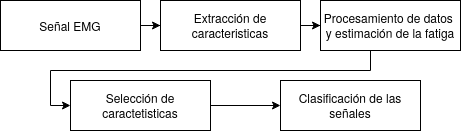
\includegraphics[scale=0.7]{imagenes/diagrma simple.png}
    \caption{ Pipeline del proyecto }
    \label{fig:esuqmemaarchivo}
    \end{figure}
 
\newpage   
\section{Obtención de las señales EMG}
Los datos utilizados para la realización del proyecto han sido tomados y filtrados con el electromiógrafo de mDurance ya comentado en secciones anteriores. Este electromiógrafo consta de 4 canales, por lo que se han podido analizar el rendimiento de 4 músculos, 2 de ellos de la extremidad inferior derecha y otros 2 de la extremidad inferior izquierda. Con esto lo que se ha obtenido son los datos de las señales de electromiografía asociados a unas pruebas. Para la obtención de los datos se tomó un conjunto de personas, que realizaron 6 series de 12 repeticiones de sentadillas con un peso relativo al 70 por ciento del RM (repetición máxima) de cada persona. Las 6 series fueron repartidas en dos días diferentes, es decir, 3 series por día, siendo estos días no consecutivos. 

También se registraron las velocidades de cada repetición. Con las velocidades de cada repetición y partiendo de la condición explicada en el análisis del problema (ver \ref{velo condicion}), se pueden estimar las repeticiones en donde los sujetos experimentaron fatiga y utilizar todos estos datos para el desarrollo de nuestro modelo de clasificación.


\section{Estimación del tamaño de ventana}
Los datos obtenidos comentados anteriormente y facilitados por mDurance, constan de señales de electromiografía brutas. Para obtener información relevante de estas señales EMG primeramente hace falta estimar el tamaño de ventana de cada una de las repeticiones registradas en las señales. 

Para ello se ha hecho uso de un proceso de detección de la actividad muscular a partir de una señal EMG, para así poder detectar fácilmente los tramos de la señal representativos de cada repetición y poder asociar a cada repetición su correspondiente estado de fatiga, analizando su velocidad registrada. Además con el diseño de dividir una señal EMG en sus diferentes activaciones (ventana de activación), nos aseguramos que los datos obtenidos son reales y más precisos, ya que solo tiene el valor de cada repetición y eliminamos el ruido que ha podido ser producido a la hora de situar o quitar el electromiógrafo.

Además se llevó a cabo una selección de los archivos de EMG más útiles, ya que ciertos archivos, vienen con mucho ruido externo y no se llega a detectar las 12 repeticiones claramente.
\section{Extracción de características}
 Una vez se ha estimado el tamaño de ventana de cada una de las repeticiones, el siguiente paso es la extracción de las características de la señal de cada una de las repeticiones registradas. Para ello con la estimación del tamaño de ventana podemos obtener unas características con unos valores muy fiables. 

 Existen un gran número de características, tanto en el dominio del tiempo, como en el dominio de la frecuencia. En este caso se han estudiado 15 características diferentes. (Para la obtención de conocimientos sobre estas características así como sus funciones se ha hecho uso de \cite{romo2007analisis,phinyomark2012feature}).

Con respecto a las características del dominio del tiempo he investigado sobre:

\begin{itemize}
\item Root mean square (RMS) \cite{phinyomark2012feature}:

    \begin{figure}[ht]
        \centering
        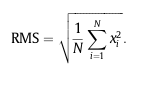
\includegraphics[scale=0.8]{imagenes/formula de caracteristicas/rms.png}
        \caption{ Definición de RMS \cite{phinyomark2012feature}}
        \label{fig:rms1}
    \end{figure}


\item Mean absolute value (MAV) \cite{phinyomark2012feature}:

    \begin{figure}[ht]
        \centering
        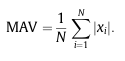
\includegraphics[scale=0.8]{imagenes/formula de caracteristicas/mav.png}
        \caption{ Definición de MAV \cite{phinyomark2012feature}}
        \label{fig:mav1}
    \end{figure}
    
 \newpage   
\item Zero crossing (ZC) con umbral de 0,01 \cite{phinyomark2012feature}:
    \begin{figure}[ht]
        \centering
        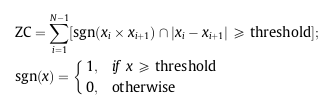
\includegraphics[scale=0.8]{imagenes/formula de caracteristicas/zc.png}
        \caption{ Definición de ZC \cite{phinyomark2012feature}}
        \label{fig:zc1}
    \end{figure}


\item Waveform length (WL) \cite{phinyomark2012feature}:
    \begin{figure}[ht]
        \centering
        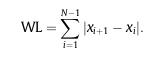
\includegraphics[scale=0.8]{imagenes/formula de caracteristicas/wl.png}
        \caption{ Definición de WL \cite{phinyomark2012feature}}
        \label{fig:wl1}
    \end{figure}

\item Slope sign change (SSC) con umbral de 0,01 \cite{phinyomark2012feature}:
    \begin{figure}[ht]
        \centering
        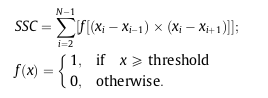
\includegraphics[scale=0.8]{imagenes/formula de caracteristicas/ssc.png}
        \caption{ Definición de SSC \cite{phinyomark2012feature}}
        \label{fig:ssc1}
    \end{figure}
   
\item Integrated EMG (IEMG) \cite{phinyomark2012feature}:
    \begin{figure}[!ht]
        \centering
        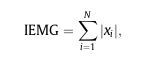
\includegraphics[scale=0.8]{imagenes/formula de caracteristicas/iemg.png}
        \caption{ Definición de IEMG \cite{phinyomark2012feature}}
        \label{fig:iemg1}
    \end{figure}
\newpage
\item Simple square integral (SSI) \cite{phinyomark2012feature}:
    \begin{figure}[!ht]
        \centering
        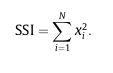
\includegraphics[scale=0.8]{imagenes/formula de caracteristicas/ssi.png}
        \caption{ Definición de SSI \cite{phinyomark2012feature}}
        \label{fig:ssi1}
    \end{figure}
    

\item Variance of EMG (VAR) \cite{phinyomark2012feature}:
    \begin{figure}[ht]
        \centering
        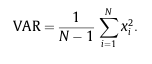
\includegraphics[scale=0.8]{imagenes/formula de caracteristicas/var.png}
        \caption{ Definición de VAR \cite{phinyomark2012feature}}
        \label{fig:var1}
    \end{figure}
    
    
    
\item Absolute value 3rd (TM3) \cite{phinyomark2012feature}:
    \begin{figure}[!ht]
        \centering
        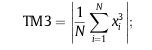
\includegraphics[scale=0.8]{imagenes/formula de caracteristicas/tm3.png}
        \caption{ Definición de TM3 \cite{phinyomark2012feature}}
        \label{fig:tm31}
    \end{figure}
    

\item Absolute value 4th (TM4) \cite{phinyomark2012feature}:
    \begin{figure}[!ht]
        \centering
        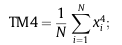
\includegraphics[scale=0.8]{imagenes/formula de caracteristicas/tm4.png}
        \caption{ Definición de TM4 \cite{phinyomark2012feature}}
        \label{fig:tm41}
    \end{figure}
\item Absolute value 5th (TM5) \cite{phinyomark2012feature}:
    \begin{figure}[!ht]
        \centering
        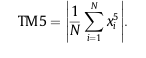
\includegraphics[scale=0.8]{imagenes/formula de caracteristicas/tm5.png}
        \caption{ Definición de TM5 \cite{phinyomark2012feature}}
        \label{fig:tm51}
    \end{figure}
    
\newpage
\item Log detector (LOG) \cite{phinyomark2012feature}:
    \begin{figure}[!ht]
        \centering
        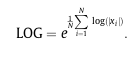
\includegraphics[scale=0.8]{imagenes/formula de caracteristicas/log.png}
        \caption{ Definición de LOG \cite{phinyomark2012feature}}
        \label{fig:log1}
    \end{figure}
    
\item Average amplitude change (ACC) \cite{phinyomark2012feature}:
    \begin{figure}[!ht]
        \centering
        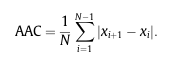
\includegraphics[scale=0.8]{imagenes/formula de caracteristicas/acc.png}
        \caption{ Definición de ACC \cite{phinyomark2012feature}}
        \label{fig:acc1}
    \end{figure}
\end{itemize}

Con respecto al dominio de la frecuencia he investigado sobre:
\begin{itemize}
\item Median frecuency (MDF) \cite{phinyomark2012feature}:
    
    \begin{figure}[!ht]
        \centering
        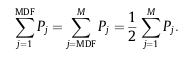
\includegraphics[scale=0.8]{imagenes/formula de caracteristicas/mdf.png}
        \caption{ Definición de MDF \cite{phinyomark2012feature}}
        \label{fig:mdf1}
    \end{figure}

\item Mean frecuency (MNF) \cite{phinyomark2012feature}:
    \begin{figure}[!ht]
        \centering
        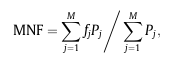
\includegraphics[scale=0.8]{imagenes/formula de caracteristicas/mnf.png}
        \caption{ Definición de MNF \cite{phinyomark2012feature}}
        \label{fig:mnf1}
    \end{figure}
\end{itemize}

\newpage
\section{Estimación de fatiga}
Para estimar la fatiga, como ya se ha comentado en capítulos anteriores, el proyecto se ha basado en que una vez que se registra una velocidad que decae un 20 por ciento, con respecto a la velocidad de la primera repetición y esto se cumple en dos repeticiones seguidas, se considera que el atleta ha entrado en fatiga y la repetición en cuestión analizada y todas las siguientes se etiquetarán como fatiga.


\section{Selección de características: RFE}
Para dotar al clasificador de una mayor simpleza y un mejor rendimiento tanto a la hora de clasificar como en tiempo de ejecución, se ha utilizado un algoritmo para estimar que características de todas las estudiadas anteriormente son las más representativas de la fatiga. Se ha hecho uso del algoritmo Recursive Feature Elimination (RFE) \cite{ramos2018emg}. Este algoritmo parte del dataset completo y en cada iteración elimina la característica menos representativa, hasta que se alcanza el número de características deseado. Con el uso de este algoritmo se han obtenido tres tipos de dataset con diferente número de variables para realizar el estudio. En este caso fueron estudiados con 1 característica, con 2 características y con 5 características. Por lo que finalmente obtendremos un gran número de resultados para realizar las conclusiones oportunas. El esquema final de todos los dataset que serán analizados es el siguiente (Ver \ref{fig:esquemageneral}).


\section{Clasificación binaria de señales}
Una vez realizada toda la fase de extracción y selección de características, debemos de realizar el diseño de los clasificadores. Para nuestro problema de clasificación binaria, donde 1 es identificador de fatiga y 0 es identificador de no fatiga, hemos estudiado el rendimiento de tres clasificadores. Se trata de 3 conjuntos de algoritmos de aprendizaje supervisado donde es necesario un conjunto de datos para el entrenamiento del modelo y otro conjunto de datos no conocido por el modelo, para estudiar su rendimiento a la hora de clasificar. A continuación se explica el funcionamiento y diseño de cada uno de ellos.
    \newpage
    \subsection{Support vector machines (SVMs): máquinas de vector de soporte}
    Su clasificación reside en que se construye un modelo que es capaz de predecir a que subgrupo de los dos, pertenece un nuevo punto del cual no conocemos su categoría.
    Para ello lo que se realiza es la obtención de un hiperplano que divida el conjunto de datos iniciales en dos grupos bien diferenciados. Los vectores de soporte son los encargados de definir el espacio de separación entre el hiperplano y las dos clases en cuestión (1,0). Cuanto mayor sea el margen entre los vectores de soporte de cada clase y el hiperplano, mejor será el modelo, ya que tendrá más claro donde clasificar datos futuros. Para el diseño del modelo se ha utilizado el kernel tipo sigmoide.
    
    \begin{figure}[ht]
    \centering
    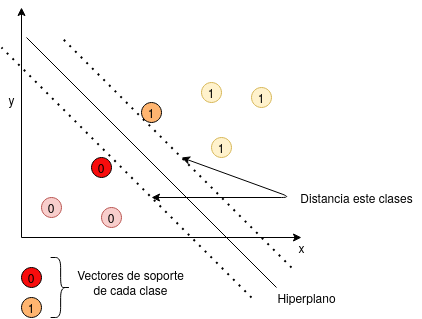
\includegraphics[width=1.0\textwidth]{imagenes/svm.png}
    \caption{ Esquema sobre funcionamiento del clasificador SVM }
    \label{fig:svm}
    \end{figure}
    
    \newpage
    \subsection{Decision trees (Trees): árboles de decisión}
    Los árboles de decisión son unos de los métodos más populares en machine learning debido a su gran eficiencia y sencillez. Se trata de un algoritmo de aprendizaje supervisado. Se puede entender como un árbol general formado por subárboles, donde cada nodo raíz de cada subárbol es una condición y las hojas de dichos subárboles, las etiquetas. El algoritmo selecciona las características del dataset más influyentes y va dividiendo el dataset completo en subconjuntos de datos, por lo que, dichas características formarán parte de los nodos de decisión, hasta que todos los nodos del árbol sean nodos hoja.
    
    
    \begin{figure}[!ht]
    \centering
    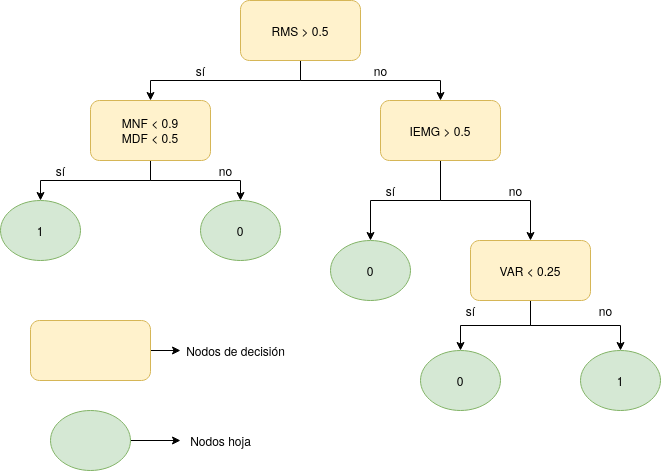
\includegraphics[width=1.0\textwidth]{imagenes/arboles de decision.png}
    \caption{ Esquema sobre funcionamiento del árbol de decisión }
    \label{fig:arbol}
    \end{figure}
    
 
  
    \subsection{K nearest neighbors (KNN): K vecinos más cercanos}
    Este algoritmo de clasificación opera de una forma muy sencilla. Se basa en estimar la categoría de un dato nuevo, en base a la categoría de sus K vecinos más cercanos. De estos K vecinos más cercanos sí conoce su categoría debido a que forman parte del conjunto de datos de entrenamiento. Debido a esto el valor de K que sea utilizado influirá mucho en el rendimiento de nuestro clasificador. El valor de K que se ha utilizado para este proyecto es de 6 vecinos.
    \begin{figure}[!ht]
    \centering
    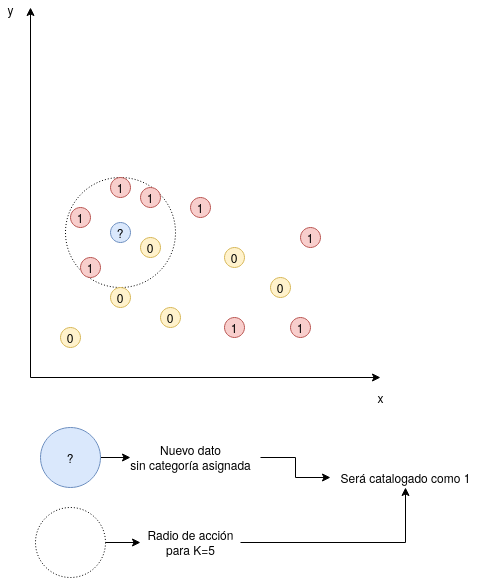
\includegraphics[width=1.0\textwidth]{imagenes/KNN.png}
    \caption{ Esquema sobre funcionamiento del KNN para K = 5 }
    \label{fig:knn}
    \end{figure}
    \section{Estudio del rendimiento obtenido: validación cruzada}
    Para validar el rendimiento de los tres clasificadores expuestos anteriormente se ha hecho uso de la validación cruzada. Con esto, sobre un mismo archivo de entrenamiento-testeo obtenemos diferentes conjuntos de datos para evaluar y testear el clasificador. En cada iteración el modelo se entrena con una parte diferente del conjunto de datos del archivo entrenamiento-testeo y con la parte restante se realiza el testeo. (Ver \ref{fig:validacioncruzada}).
    
    Se obtendrá una serie de precisiones, una por cada iteración de la validación cruzada, y podremos obtener una precisión media del clasificador y una desviación estándar, que nos dará una idea de cuanto de bueno es nuestro clasificador. Para el diseño de nuestra validación cruzada se ha utilizado un valor de k = 15.
    
    \begin{figure}[ht]
    %\centering
    \includegraphics[width=1.0\textwidth, height=10cm]{imagenes/validación cruzada.png}
    \caption{ Validación cruzada para k = 5  }
    \label{fig:validacioncruzada}
    \end{figure}
    
    
\section{Procesamiento de datos: diferentes modelos de estudio} \label{tiposClasificadores}
El electromiógrafo utilizado para la medición de la actividad muscular a la hora de realizar las sentadillas consta de 4 canales diferentes. (Ver Imagen \ref{fig:esquemaarchivoEMG}).
\begin{itemize}
\item Canal 1: registra la actividad muscular del vasto medial de la pierna izquierda.
\item Canal 2: registra la actividad muscular del recto femoral de la pierna izquierda.
\item Canal 3: registra la actividad muscular del vasto medial de la pierna derecha.
\item Canal 4: registra la actividad muscular del recto femoral de la pierna derecha.
\end{itemize}
Debido a la gran ventaja que nos aporta la herramienta utilizada se ha optado por realizar diferentes tipos de archivos de entrenamiento-testeo y ver cual de ellos sería el más indicado a la hora de resolver nuestro problema. Cada uno de los archivos de entrenamiento-testeo que se van a describir a continuación están formados mediante la agrupación de los diferentes canales. Con esto se pretende simular diferentes situaciones y ver cual de ellas sería la más indicada para resolver el proyecto.



A continuación se muestra un esquema resumen sobre los archivos EMG utilizados y sus características extraídas. Con estos datos se formarán los archivos de entrenamiento-testeo.


    \begin{figure}[!ht]
    \centering
    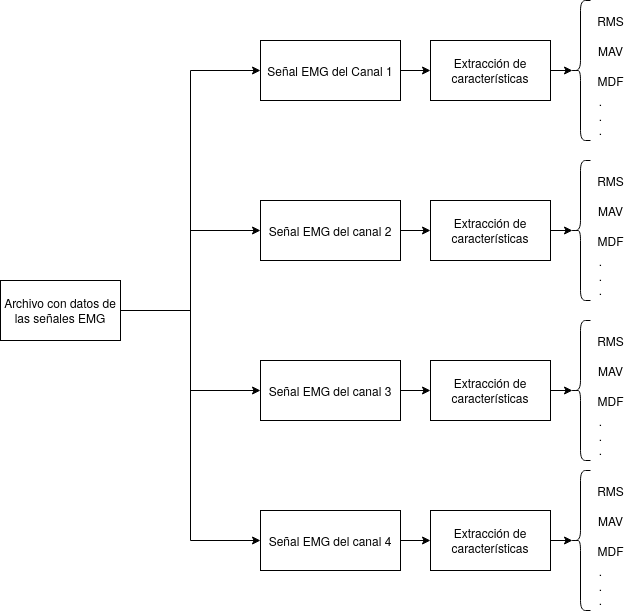
\includegraphics[width=0.94\textwidth]{imagenes/esquema de los canales.png}
    \caption{ Esquema de archivo EMG bruto: 1 serie de 12 repeticiones de sentadillas }
    \label{fig:esquemaarchivoEMG}
    \end{figure}



    \subsection{Canal 1, canal 2, canal 3, canal 4}
La primera idea llevada a cabo es implementar un clasificador para cada canal. Con esto lo que se obtendría es una precisión muscular muy alta a la hora de detectar la fatiga muscular. Es decir, a la hora de realizar una serie de sentadillas podríamos averiguar que músculo de los 4 registrados es el que entra en fatiga. Para ello se han diseñado 4 tipos de archivos de entrenamiento-testeo. Los 4 tipos de archivos tienen la misma organización, lo único que cambia entre ellos es el valor que contienen. Por ejemplo, el archivo del canal 1, solo contiene los valores de las características extraídas de las señales EMG del vasto medial izquierdo. Para ello cada columna del dataset es identificada por cada una de las 15 características estudiadas, siendo la última columna, la representación de la fatiga asociada a cada repetición. Con respecto a las filas, las 12 primeras filas corresponden a las 12 repeticiones del primer archivo EMG analizado, las 12 siguientes a las 12 repeticiones del segundo archivo, etc. 

Esto se puede aplicar también a los canales 2, 3 y 4. El esquema para el archivo de entrenamiento-testeo del canal N siendo N={1, 2, 3, 4} y de cada archivo K siendo K={1, 2, ..., 19} (número total de archivos analizados) es:

\begin{figure}[ht]

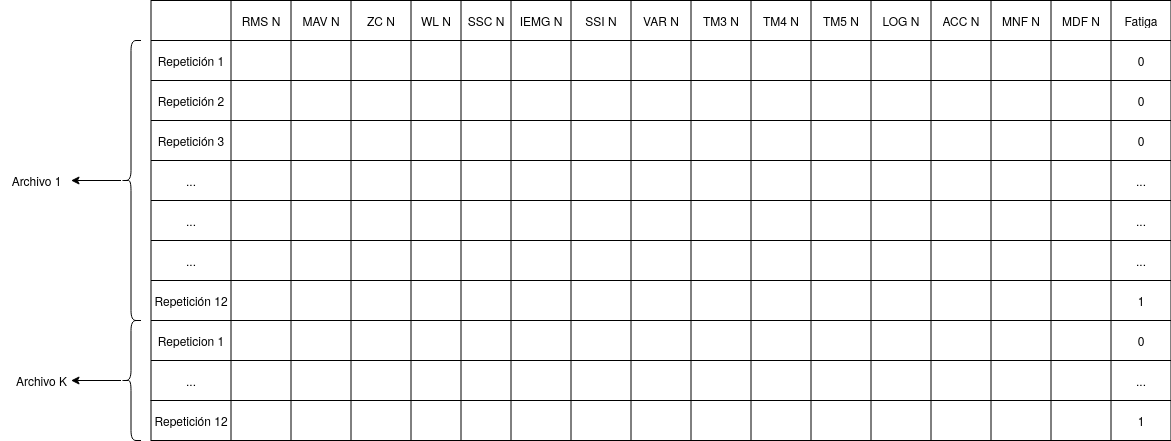
\includegraphics[width=1.0\textwidth,height=7cm]{imagenes/canal1234.png}
\caption{ Esquema de archivo de entrenamiento-testeo para cada canal 1, 2, 3, 4}
\label{fig:canal1234}
\end{figure}


\newpage
    \subsection{Canal 1,2 y canal 3,4}
Debido a que la sentadilla es un ejercicio multiarticular e implica a las dos extremidades inferiores, la segunda idea consta de diseñar un clasificador para cada extremidad. Con esto tendremos un nivel de especificidad a nivel de extremidad y podremos detectar que extremidad inferior se fatiga antes, si la izquierda o la derecha. Para ello en esta ocasión tenemos dos archivos de entrenamiento-testeo, uno de cada extremidad. Lo que se ha llevado a cabo es la agrupación de los datos recolectados por el canal 1 y canal 2 (extremidad izquierda) y por el canal 3 y canal 4 (extremidad derecha). A continuación se muestra una breve explicación de cada archivo, así como su correspondiente esquema.

        \subsubsection{Canal 1,2: extremidad izquierda}
        Como se ha comentado anteriormente, este archivo de entrenamiento-testeo consta de los datos agrupados del canal 1 y del canal 2. En este caso el número de filas aumenta, ya que tratamos las repeticiones del canal 1 y las repeticiones del canal 2. Su esquema es el siguiente (Ver \ref{fig:canal12}).
        
        \begin{figure}[!ht]
        
        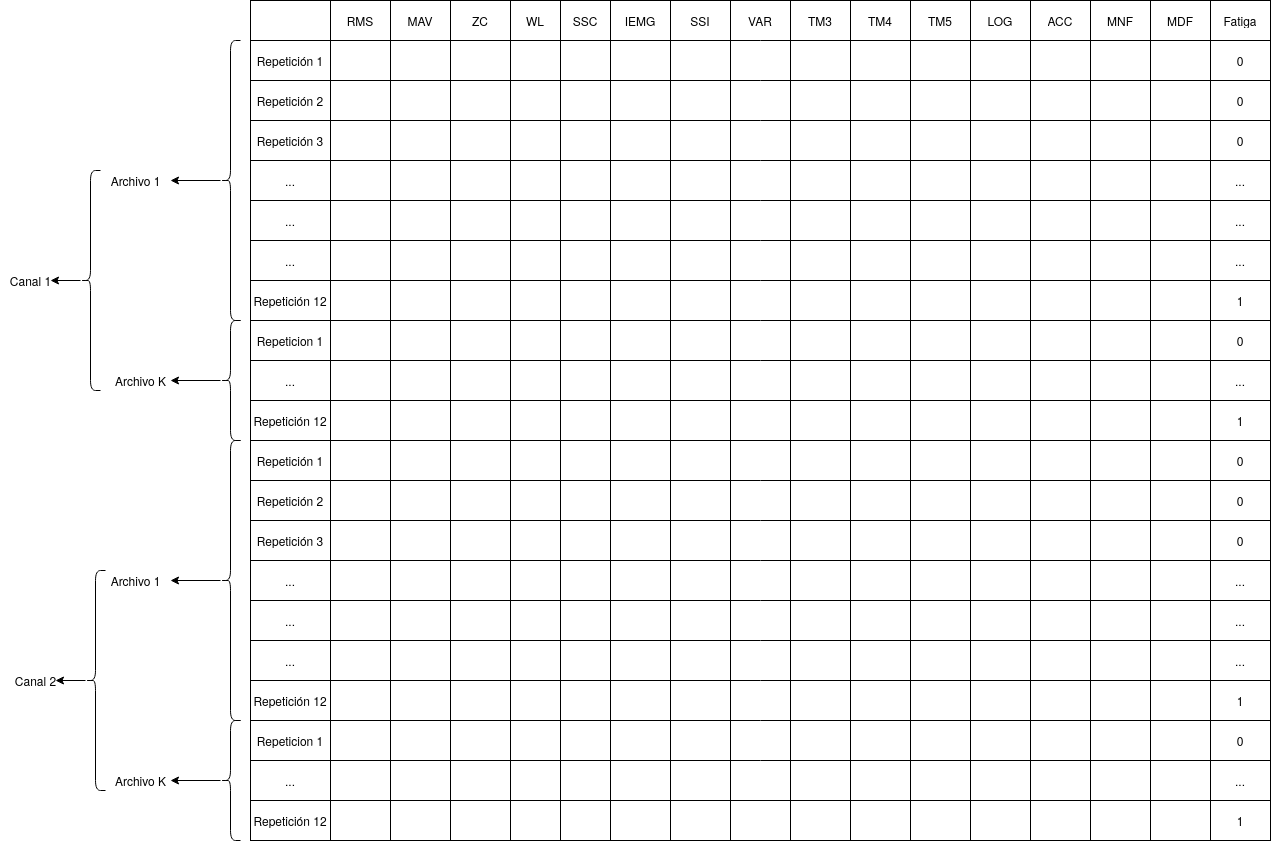
\includegraphics[width=1.0\textwidth,height=9cm]{imagenes/canal 12.png}
        \caption{ Esquema de archivo de entrenamiento-testeo para el canal 1,2}
        \label{fig:canal12}
        \end{figure}
        
        
        \newpage
        \subsubsection{Canal 3,4: extremidad derecha}
        El archivo de entrenamiento-testeo del clasificador de la extremidad derecha, es similar al de la extremidad izquierda. La única diferencia es que en este caso se agrupan los datos del canal 3 y del canal 4. Su esquema es el siguiente (Ver \ref{fig:canal34}).
        \begin{figure}[!ht]
        \centering
        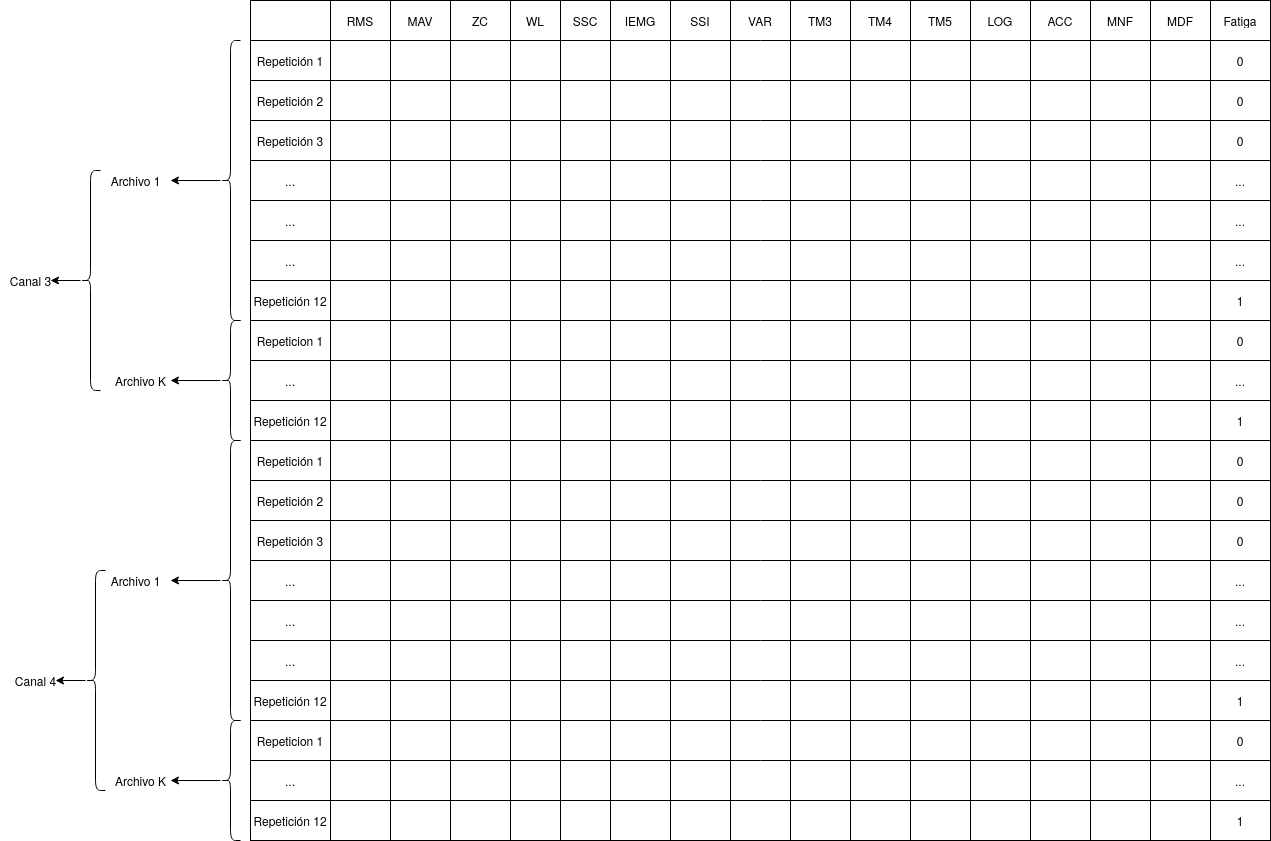
\includegraphics[width=1.0\textwidth,height=9cm]{imagenes/canal 34.png}
        \caption{ Esquema de archivo de entrenamiento-testeo para el canal 3,4}
        \label{fig:canal34}
        \end{figure}
        
    
    
    \subsection{Canal total}
    Por último, se ha pensado en el diseño de un clasificador que ha sido denominado total, donde se hallará la fatiga global del individuo en cuestión. Para ello se agruparán los datos de los 4 canales utilizados en un mismo archivo de entrenamiento-testeo. En este caso el número de filas aumenta, debido a que tenemos en conjunto la información de todos los canales. El esquema de dicho archivo es el siguiente (Ver \ref{fig:canaltotal}).


    \begin{figure}[ht]
    \centering
    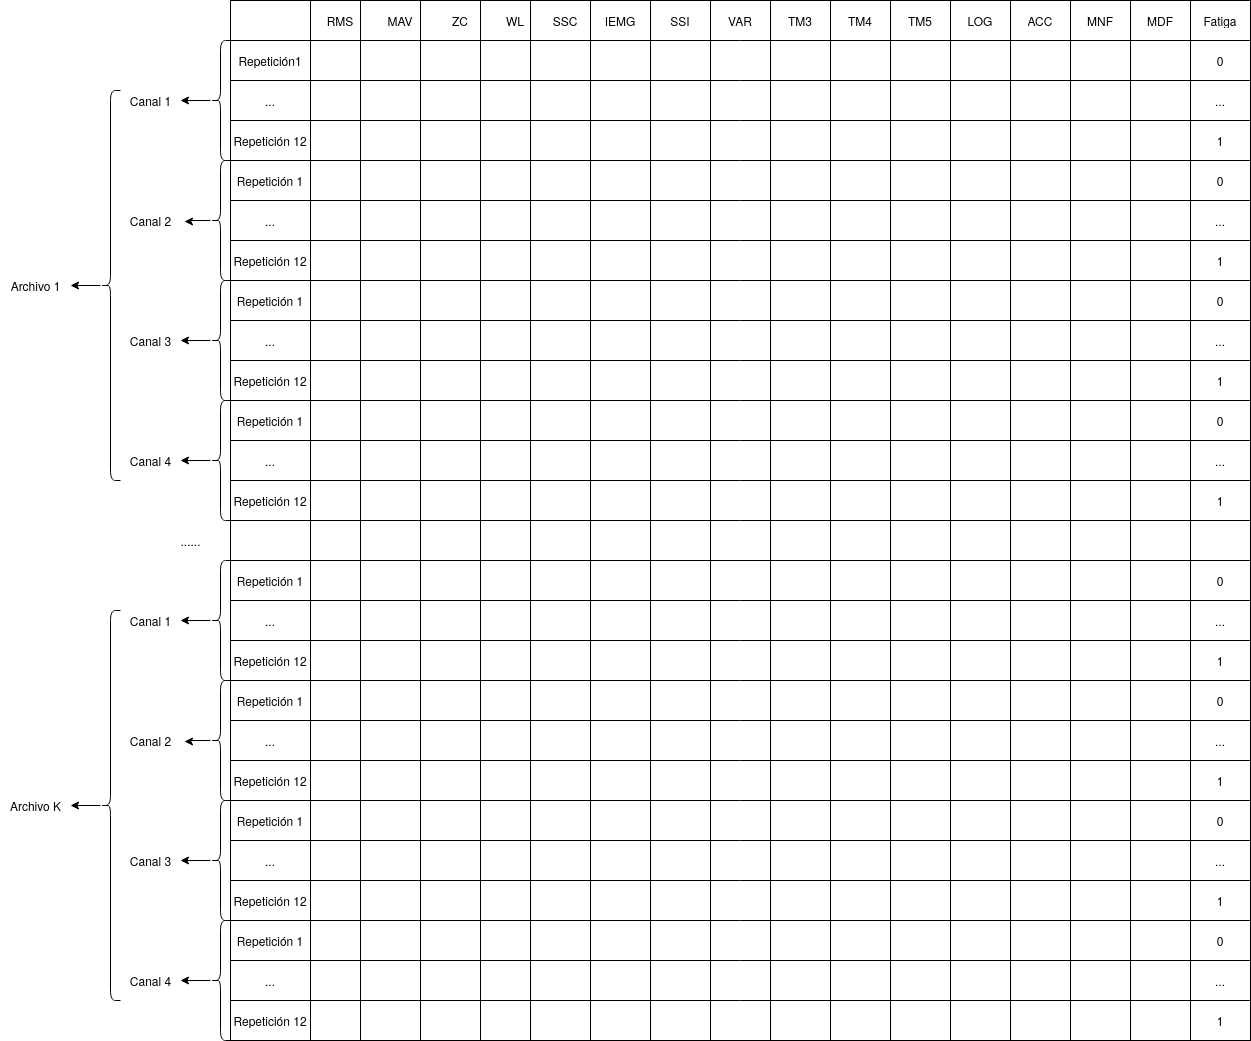
\includegraphics[scale=0.28]{imagenes/canal total.png}
    \caption{ Esquema de archivo de entrenamiento-testeo para el canal total }
    \label{fig:canaltotal}
    \end{figure}

    
        \newpage
    
\section{Esquema final del estudio}
Para finalizar la fase de metodología se pretende mostrar un esquema final sobre los diferentes tipos de clasificadores finales. El objetivo es analizar cuál sería el número óptimo de características (N=1,2,5 ) y el tipo de clasificador (SVM, Tree, KNN) para cada uno de los canales que son estudiados (canal 1, canal 2, canal 3, canal 4, canal (1,2), canal (3,4), canal total). Ver sección \ref{tiposClasificadores} para mayor detalle. (Ver esquema \ref{fig:esquemageneral}).



 \begin{figure}[h]
    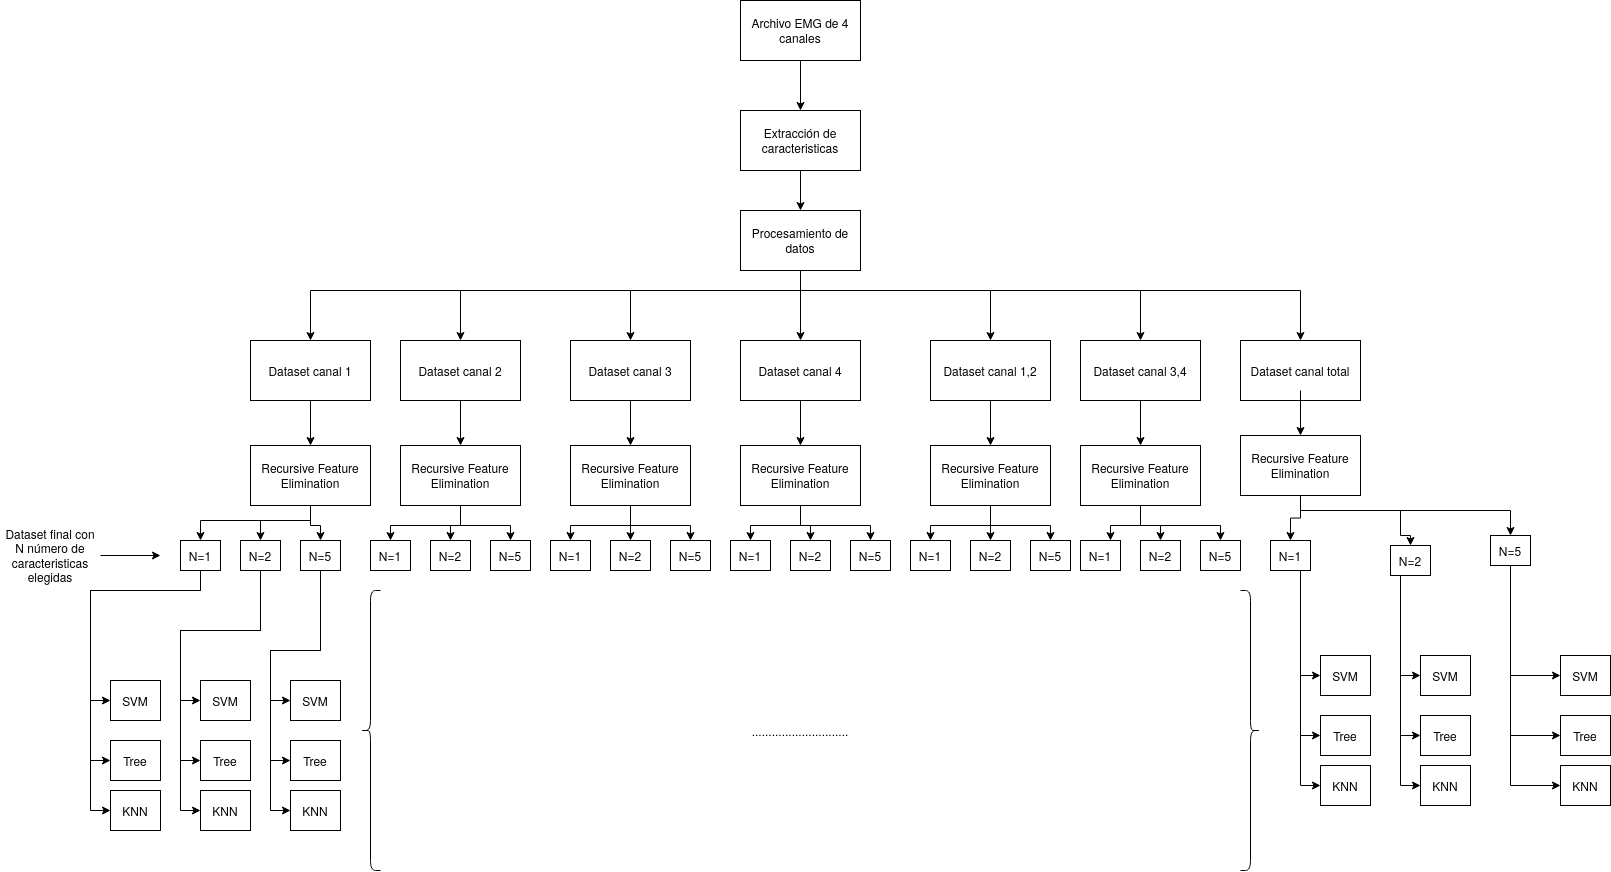
\includegraphics[height=0.85\textwidth,angle=90]{imagenes/esquema final.png}
    \caption{ Esquema general del sistema }
    \label{fig:esquemageneral}
   \end{figure}
    

